\documentclass[a4paper,12pt]{article}
\usepackage{graphicx}
\usepackage{hyperref} 
\usepackage{enumitem}
\usepackage{makecell}
\usepackage{amsmath}
\usepackage{amssymb}
\usepackage{gensymb}
\usepackage[T1]{fontenc}
\usepackage{fancyhdr}
\usepackage{caption}
\usepackage{subcaption}
\usepackage[utf8]{inputenc}
\usepackage[english]{babel}
\usepackage{hyperref}
\hypersetup{
    colorlinks=false,
    linkbordercolor=0 1 1,
    filecolor=magenta,      
    urlcolor=cyan,
}
%\usepackage[shortlabels]{enumerate}

\graphicspath{ {/home/nareshguru77/Documents/learning_materials/Semester_2/RandD/semantic_segmentation/proposal/texmaker} }

%\usepackage[letterpaper, portrait, margin=0.6in]{geometry}

\title{R$\&$D Project Proposal\\ \vspace{5mm}Semantic Segmentation using Resource Efficient Deep Learning}
\author{Naresh Kumar Gurulingan\footnote{naresh.gurulingan@smail.inf.h-brs.de}}
%Matrikel Nr.: 
%\date

\begin{document}
\begin{titlepage}
	\begin{center}
		
	\end{center}
	\begin{center}
		\begin{LARGE}
			R$\&$D Project Proposal\\
			\vspace{5mm}
			Semantic Segmentation using Resource Efficient Deep Learning
		\end{LARGE}
	\end{center}
	\begin{center}
		Naresh Kumar Gurulingan\\
		Matrikel Nr.: 9030384
	\end{center}
	
	\begin{center}
		B-IT Master Studies Autonomous Systems\\
		\vspace{5mm}
		University of Applied Sciences Bonn-Rhein-Sieg\\
		Advisor: Prof. Dr. Paul G. Pl{\"o}ger\\
		Second Advisor: M. Sc. Deebul Nair\\
		\vspace{5mm}
		November 23, 2017
\end{center}

\begin{large}
	\begin{center}
		\textbf{Abstract}
	\end{center}
\end{large}
\hspace{8mm}Semantic Segmentation is a computer vision task in which an image is split into meaningful regions such that each region represents a different object or background. In the context of deep learning, semantic segmentation is treated as a pixelwise classification problem where a neural network is trained to assign a class to every pixel in the input image. Existing state-of-the-art methods repurpose image classification pretrained Convolutional Neural Network architectures for semantic segmentation. This enables the transfer of learned representations from CNNs which show excellent performance in image classification.\\

Therefore, the underlying CNN architecture is often a deep image classification model with large number of free parameters and slow inference times. This makes the semantic segmentation networks unsuitable for mobile or embedded devices because of the high demand on memory and computational power. Several approaches have been proposed in the literature to reduce the resource requirements of CNN architectures. This work aims to analyze the feasibility of using such approaches in current state-of-the-art semantic segmentation networks without considerably affecting the accuracy.

\end{titlepage}
\tableofcontents

\newpage
\section{Introduction}
\hspace{8mm}In recent years, deep learning has significantly impacted research in the field of computer vision. Variations of Convolutional Neural Network architectures have shown state-of-the-art performance in computer vision tasks such as image classification \cite{1}, object detection \cite{2}, action recognition \cite{3} and semantic segmentation \cite{4}. A considerable part of this success comes from the supervised learning paradigm through which the networks are trained with labeled samples.\\

State-of-the-art deep learning techniques in semantic segmentation also make use of the supervised learning paradigm. Semantic segmentation is treated as a pixelwise classification problem with the goal of assigning a class from a list of desired classes to every pixel in an image. The resultant image splits objects of interest into different regions thereby achieving the intended segmentation in a meaningful manner.\\
\begin{center}
	\begin{figure}[!htb]
		\begin{subfigure}{.5\textwidth}
			\centering
			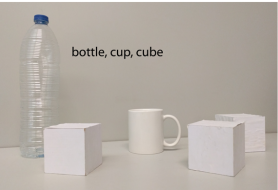
\includegraphics[width=.7\linewidth]{image_classification.png}
			\caption{Image classification}
			\label{Fig:1a}
		\end{subfigure}
		\begin{subfigure}{.5\textwidth}
			\centering
			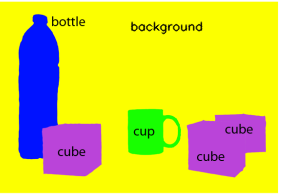
\includegraphics[width=.7\linewidth]{semantic_segmentation.png}
			\caption{Semantic Segmentation}
			\label{Fig:1b}
		\end{subfigure}
		\caption{Illustration of Image Classification and Semantic Segmentation\cite{5}}
	\end{figure}
\end{center}

However, unlike the task of image classification[\ref{Fig:1a}], where the location and boundaries of the desired object in the image is irrelevant, semantic segmentation[\ref{Fig:1b}] requires the neural network to be able to spatially localize desired objects and its boundaries. Also, image classification networks are only required to produce probability scores to different desired classes based on the input image whereas a semantic segmentation network is required to produce a single channel segmentation map which is of the same size as the input image.\\

Despite these differences, state-of-the-art approaches adopt image classification networks and repurpose them for semantic segmentation. One reason for this adoption is to avoid much of the overhead involved in training the network from scratch. Another reason is concerned with the difficulty in obtaining datasets for semantic segmentation because of the need to annotate every pixel to obtain ground truth. This difficulty is apparent when the number of fine annotated images in the commonly used Cityscapes dataset (5000 fine annotated images) for semantic segmentation is compared with ImageNet dataset (over a million labeled images) for image classification. In light of this difficulty, it makes sense to make use of the transfer learning approach to transfer learned representations from the image classification pretrained networks to semantic segmentation networks. This enables the use of large networks though only a limited amount of training data is available.\\

The underlying image classification networks often contain a large number of layers and free parameters leading to high memory requirements. This makes them unsuitable for embedded or mobile devices where memory available in limited. Also, real time performance is hindered because the networks are computationally heavy. These drawbacks can be addressed by using strategies proposed in the literature such as pruning, quantization and others. The goal of this work is to make use of such strategies on state-of-the-art semantic segmentation networks to obtain a lean model suitable for application in an embedded setting.

\section{Related Work}
The related works can be broadly grouped into three categories:
\begin{enumerate}
	\item Accuracy.
	\item Strategies for DCNN efficiency.
	\item Accuracy and resource efficiency.
\end{enumerate}
\subsection{Improving accuracy}
This section addresses deep learning semantic segmentation models which focus on accuracy and not on the resource requirements. \\
\begin{itemize}
	\item Fully Convolutional Network:\cite{5} \\
		A popular approach which belongs to this category is the Fully Convolutional Network\cite{6} which replaces the last few fully connected layers of image classification pretrained CNNs with convolutional layers for the purpose of semantic segmentation. Information from the lower pooling layers are combined with the final prediction to improve the fineness of the segmentation. The authors call this as skip architecture. The major drawback however is the lack of global context awareness due to the downsampling operations which make the network spatially invariant. The importance of global context can be stated with an example. For instance in the figure \ref{Fig:1a}, it can be seen that a set white pixels, when looked at locally, could either belong to the cube or the cup. Only when looked at globally, it is possible to differentiate between the two.
		\item Encoder-Decoder architectures:\cite{5}\\
		In this type of architectures, the encoder creates a low resolution feature map by downsampling the input image. The decoder works on the resultant low resolution feature maps and upsamples them to the original image resolution using fractionally strided convolutions. Both the encoder and decoder contain trainable kernels. A popular example of this architecture is the SegNet\cite{7}.
		\item Approaches to integrate context knowledge:\cite{5}\\
		Since, global context awareness is significant for semantic segmentation, a number of approaches have been proposed to integrate context knowledge. \\
		One such approach is the use of Conditional Random Fields as a post processing step to make coarse predictions finer. The approach called DeepLab\cite{4}, for instance, makes use of fully connected pairwise CRF. Dilated convolutions is another approach in which the kernels are enlarged without an increase in the number of free parameters such that each kernel looks into a larger area of the feature map. DeepLab\cite{4} also uses dilated convolutions. Other approaches also make use of multi-scale aggregation, Recurrent Neural Networks.\\
\end{itemize}
This project does not intend to look into approaches in this category in detail. Rather, a subset of approaches will be selected based on criteria such as accuracy and model size.

\subsection{Strategies for DCNN efficiency}
This section addresses literature dealing with strategies to improve the resource efficiency of deep convolutional neural networks. Related approaches fall into one of the following:
\begin{itemize}
	\item Reducing the precision of weights and feature maps:\cite{8}
		\begin{enumerate}
			\item Quantization: The idea behind quantization is that reducing the FLOPS (Floating Point Operations per Second) involved during inference, would lead to faster inference times. The weights could be quantized and represented in integers thereby reducing the memory requirements. Quantizing the feature maps during inference would reduce the computation requirements. However, accuracy of the resultant network would be lower. Quantization can be done to an extent to which loss of precision does not lead to considerable accuracy loss.
			\item Weight Sharing: In weight sharing, a set of weight parameters are forced to always have the same values. This could be the weights belonging to a kernel or a entire feature map. With weight sharing, one value can be stored and the weights which share this value can just store the index of the value. This could lead to reduced storage requirements at the cost of accuracy loss.
		\end{enumerate}
	\item Reducing the model size:\cite{8}
		\begin{enumerate}
			\item Pruning: Pruning explores the possibility to removing  weights in the CNN which are redundant and do not contribute to the accuracy of the model. This leads to a reduction in the number of weights, thereby reducing memory requirements. However, this requires a strategy to determine whether a weight is redundant or not. One possible strategy is to set a feature map to zero and check whether the accuracy has changed. If the accuracy is not affected, the feature map can be removed. This process can be repeated for all feature maps. However, this is not feasible because of the sheer number of feature maps involved.  Pavlo Molchanov et al. (\cite{9}), point out that the VGG-16 net has 4224 convolutional feature maps and the discussed strategy would require $2^{4224}$ evaluations which is not possible.\\
			Therefore, a good strategy is required for pruning in order to determine the redundancy of weights.
		\end{enumerate}
\end{itemize}
A number of other techniques also exist such as the use of Huffman coding to reduce storage requirements\cite{10}. These approaches will be looked into in detail by this project.

\subsection{Accuracy and resource efficiency}
This section addresses deep learning semantic segmentation models which focus on reducing the resource requirements while maintaining accuracy. These approaches are closely related to this project. 
\begin{itemize}
	\item ENet \cite{11}: In this approach, the authors exploit certain design choices which enables them to arrive at a reduction in the resource requirements namely memory and inference time. For instance, the early layers of the network heavily reduce the input size based on the notion that visual information is spatially redundant and also that the initial layers are expected to act like good feature detectors by preprocessing the input. This design change speeds up inference time because computations in the early layers are reduced. Other design choices are also made leading to further reduction in resource consumption.
\end{itemize}
% Speeding up Semantic Segmentation for Autonomous Driving, Efficient ConvNet for real-time semantic segmentation.%ERFNet: Efficient Residual Factorized ConvNet for Real-Time Semantic Segmentation

ENet achieves considerable reduction in resource requirements, by exploring the use of alternate design choices. However, existing strategies described in Section 2.2 could also be used for the same purpose.

\section{Problem Statement}
The problems intended to be addressed in this project are listed below:
	\begin{itemize}
		\item The underlying neural network architectures used in the state-of-the-art semantic segmentation approaches are often deep with many layers and have a large number of tunable parameters (for instance, 50 layer ResNet trained on the ImageNet dataset has 25.5 million parameters \cite{8}). 
		\item This hinders the use of CNNs in embedded or mobile devices, where memory and energy consumption are strict constraints.
		\item Strategies proposed in the literature to reduce resource requirements of CNNs, often, lead to degradation in performance. So an optimal trade-off between performance in terms of an accuracy metric such as Intersection over Union(IoU), and reduction of resource requirements needs to be identified.
		\item Though current state-of-the-art approaches achieve good results, efforts to visualize the representations learned by the network seems to be minimal. Often, only the final performance achieved is emphasized and the design changes made to the CNN architecture are presented as intuitions.
	\end{itemize}
An outline of the approach this project intends to take is given below:
	\begin{itemize}
		\item Different strategies have been proposed in the literature to improve the efficiency of CNNs and make them suitable for embedded or mobile devices, namely pruning \cite{9}, quantization \cite{12}. This project aims to identify such strategies and comparatively analyze their effects.
		\item The approach by \cite{13}, apply pruning on CNN architectures used for image classification (AlexNet, GoogleNet and SqueezeNet) and analyze the effects of such algorithms.
		\item This project intends to follow a similar approach and aims to apply the identified strategies, on a set of current state-of-the-art CNN architectures used for semantic segmentation such as FCN \cite{6}, SegNet \cite{7} and ENet \cite{11} and analyze the resultant effects.
		\item This project aims to visualize at various stages of application, the effects of identified strategies on the activations of convolution filters through existing approaches such as Zeiler and Fergus \cite{14}.
	\end{itemize}

\section{Project Plan}
The work plan for this project begins on December 15th, 2017 and ends in August 15th, 2018. The total project duration is 8 months. 
\subsection{Work Packages}
	\begin{center}
		\begin{figure}[htbp]
			\begin{center}
				\caption{Work Packages}
				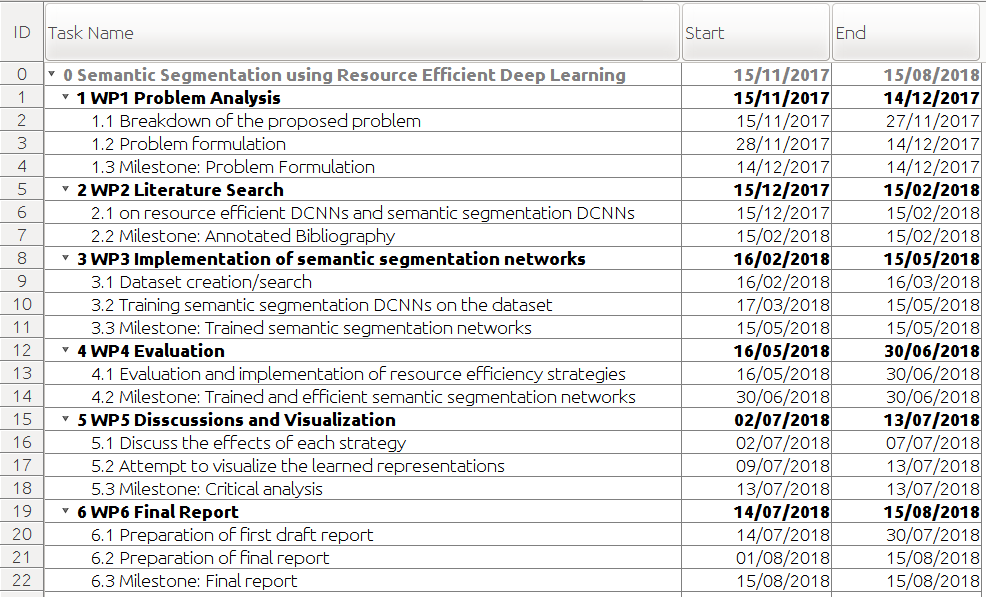
\includegraphics[scale=0.325]{workplan.png}
			\end{center}
		\end{figure}
	\end{center}

\newpage
\subsection{Gantt Chart}
	\begin{center}
		\begin{figure}[!htb]
			\begin{center}
				\caption{Gantt Chart}
				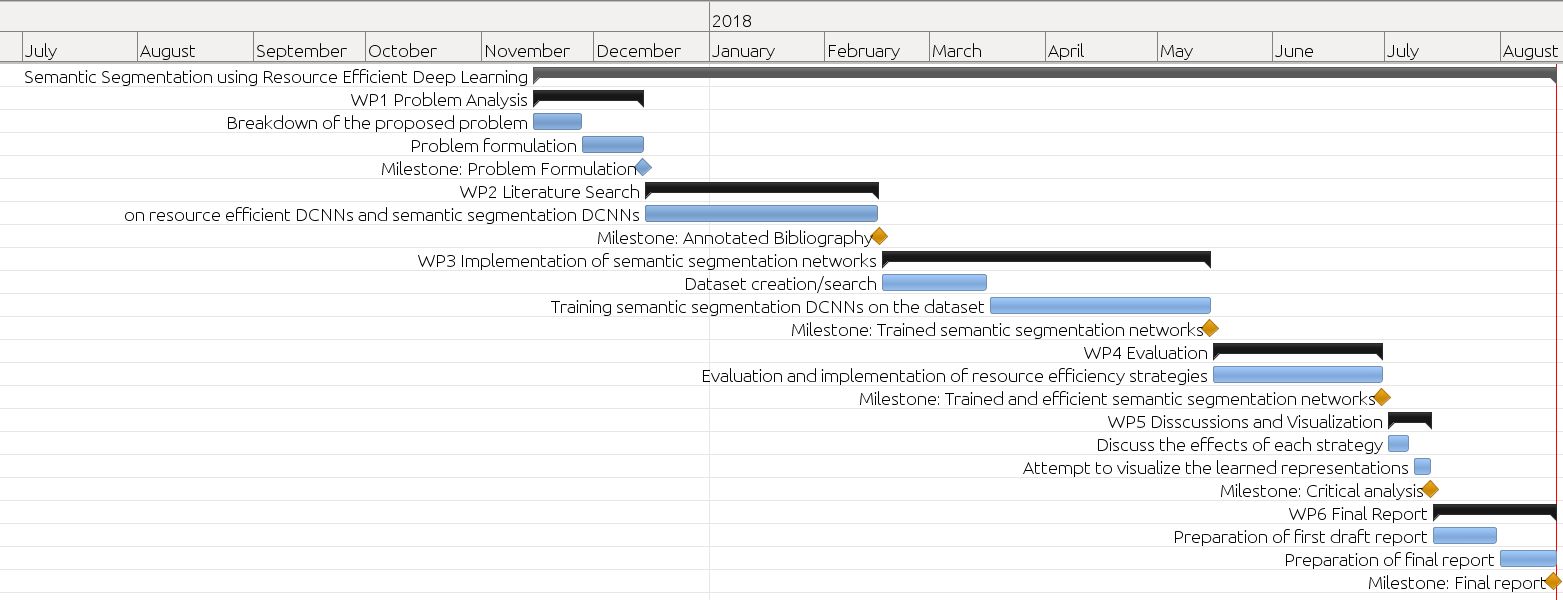
\includegraphics[scale=0.25]{gantt_chart.png}
			\end{center}
		\end{figure}
	\end{center}

\subsection{Deliverables}
\subsubsection{Minimum Viable}
	\begin{enumerate}
		\item Analysis of the current state-of-the-art strategies to improve resource efficiency of convolutional neural networks.
		\item Selection of a subset of such strategies based on feasibility of usage for convolutional neural networks trained for semantic segmentation.
	\end{enumerate}
\subsubsection{Expected}
	\begin{enumerate}
		\item Dataset creation for objects used in the Robocup @Work or Robocup @Home environment.
		\item Selection of a set of deep architectures used for semantic segmentation, fine-tuning them on the created dataset and reporting the results based on one or more performance metrics.
		\item Applying the selected resource efficiency strategies on the fine-tuned models and arriving at a trade-off between accuracy and resource consumption.
	\end{enumerate}
\subsubsection{Maximum}
	\begin{enumerate}
		\item Visualizing the learned representations of the trained networks through existing techniques such as Zeiler and Fergus \cite{14}.
		\item Integrating the resultant network with the tasks in Robocup.
		\item Further analyzing the resultant network to improve its efficiency to meet a tighter memory (<10MB) and real time (<1s) constraints (If this constraints are not already met by the resultant network).
	\end{enumerate}

\newpage
%\section{References}
\addcontentsline{toc}{section}{References}
\begin{thebibliography}{9}
\bibitem{1}
He, Kaiming and Zhang, Xiangyu and Ren, Shaoqing and Sun, Jian , "Deep residual learning for image recognition", in Proceedings of the IEEE Conference on Computer Vision and Pattern Recognition, (2016).
\bibitem{2}
Redmon, Joseph and Divvala, Santosh and Girshick, Ross and Farhadi, Ali, "You only look once: Unified, real-time object detection", in Proceedings of the IEEE Conference on Computer Vision and Pattern Recognition, (2016).
\bibitem{3}
Simonyan, Karen and Zisserman, Andrew, "Two-stream convolutional networks for action recognition in videos", in Advances in neural information processing systems, (2014).
\bibitem{4}
Chen, Liang-Chieh and Papandreou, George and Kokkinos, Iasonas and Murphy, Kevin and Yuille, Alan L , "Semantic image segmentation with Deep Convolutional Nets and fully connected CRFs", in International Conference on Learning Representations, (2016).
\bibitem{5}
Alberto Garcia-Garcia, Sergio Orts-Escolano, Sergiu Oprea, Victor Villena-Martinez, Jose Garcia-Rodriguez, "A Review on Deep Learning Techniques Applied to Semantic Segmentation", arXiv preprint	arXiv:1704.06857, 2017.
\bibitem{6}
J. Long, E. Shelhamer, and T. Darrell, "Fully convolutional networks for semantic segmentation," in Proceedings of the IEEE Conference on Computer Vision and Pattern Recognition, 2015, pp. 3431-3440.
\bibitem{7}
V. Badrinarayanan, A. Handa, and R. Cipolla, "Segnet: A deep convolutional encoder-decoder architecture for robust semantic pixel-wise labelling," arXiv preprint arXiv:1505.07293, 2015.
\bibitem{8}
Vivienne Sze, Yu-Hsin Chen, Tien-Ju Yang, Joel Emer,"Efficient Processing of Deep Neural Networks: A Tutorial and Survey", in arXiv preprint arXiv:1703.09039, 2017.
\bibitem{9}
Pavlo Molchanov, Stephen Tyree, Tero Karras, Timo Aila, Jan Kautz, "Pruning Convolutional Neural Networks for Resource Efficient Inference", in arXiv preprint arXiv:1611.06440, 2016.
\bibitem{10}
S. Han, H. Mao, and W. J. Dally, "Deep compression: Compressing deep neural networks with pruning, trained quantization and huffman coding," arXiv preprint arXiv:1510.00149, 2015.
\bibitem{11}
Adam Paszke, Abhishek Chaurasia, Sangpil Kim, and Eugenio Culurciello. , "Enet: A deep neural network architecture for real-time semantic segmentation." arXiv preprint arXiv:1606.02147, 2016.
\bibitem{12}
Jiaxiang Wu, Cong Leng, Yuhang Wang, Qinghao Hu, Jian Cheng, "Quantized Convolutional Neural Networks for Mobile Devices", in Computer Vision and Pattern Recognition, 2016.
\bibitem{13}
T.-J. Yang, Y.-H. Chen, and V. Sze, "Designing Energy-Efficient Convolutional Neural Networks using Energy-Aware Pruning," in CVPR, 2017.
\bibitem{14}
Zeiler, Matthew D. and Fergus, Rob, "Visualizing and Understanding Convolutional Networks", in Springer International Publishing, (2014).
\end{thebibliography}

\end{document}